%% Slides for ".NET Programming" by Chunyu Wang <chunyu@hit.edu.cn>

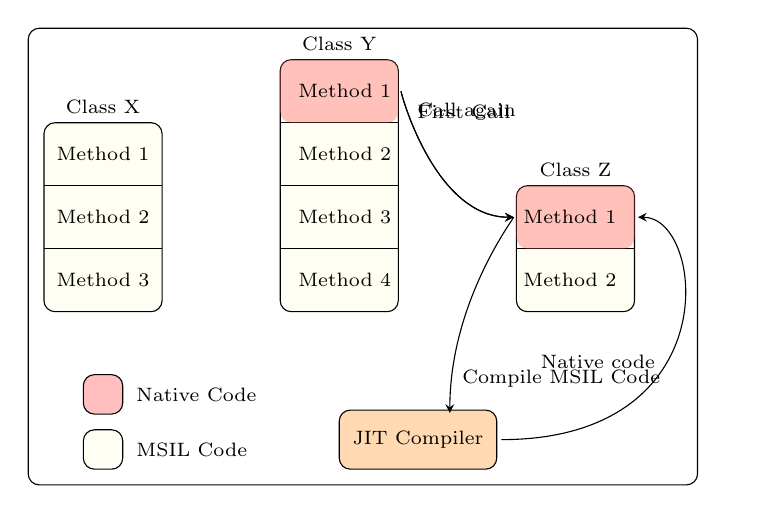
\begin{tikzpicture}[font=\scriptsize, rounded corners, >=stealth]
\def\rowstroke{++(0cm,.8cm) -- +(1.5,0)}
\draw[fill=white,fill opacity=.4] (-.2,-.2) rectangle (8.3,5.6);

\path[draw,fill=yellow!5] (0,2) rectangle +(1.5cm,.8cm*3);
\draw (0,2) \rowstroke \rowstroke;
\foreach \x in {1,2,3}\draw (0,2) +(.75cm,2.8cm-.8cm*\x) node {Method \x};
\draw (.75,4.6) node {Class X};

\path[draw,fill=yellow!5] (3,2) rectangle +(1.5cm,.8cm*4);
\draw (3,2) \rowstroke \rowstroke \rowstroke;
\fill[color=red!60,fill opacity=.4] (3cm,4.4cm) rectangle +(1.5cm,.8cm) ;
\foreach \x/\y in {1/y1,2/y2,3/y3,4/y4} \draw (3,2) +(.82cm,3.6cm-.8cm*\x) node (\y) {Method \x};
\draw (3.75,5.4) node {Class Y};

\path[draw,fill=yellow!5] (6,2) rectangle +(1.5cm,.8cm*2);
\draw (6,2) \rowstroke;
\fill<4->[color=red!60,fill opacity=.4] (6cm,2.8cm) rectangle +(1.5cm,.8cm) ;
\foreach \x/\y in {1/z1,2/z2} \draw (6,2) +(.68cm,2cm-.8cm*\x) node (\y)  {Method \x};
\draw (6.75,3.8) node {Class Z};

\fill[draw,fill=yellow!5] (.5, 0) rectangle +(.5,.5) +(.55,.25) node[anchor=west] {MSIL Code};
\fill[draw,fill=red!25]   (.5,.7) rectangle +(.5,.5) +(.55,.25) node[anchor=west] {Native Code};

\path[xshift=1cm,draw,fill=orange!30] (2.75,0) rectangle +(2,.75) +(1,.375) node (jit) {JIT Compiler};

\draw<2>[->] (y1.east) .. controls +(down:1pt) and +(left:1cm) 
.. node[near start,right] {First Call} (z1.west);
\draw<3>[->,shorten >=3pt] (z1.west) .. controls +(250:1pt) and +(up:1.5cm) 
.. node[very near end,right] {Compile MSIL Code} (jit.30);
\draw<4>[->,shorten >=.15cm, shorten <=3pt] (jit.east) .. controls +(right:3cm) and +(right:1cm)
.. node[pos=.4,left] {Native code} (z1.east);
\draw<6>[->] (y1.east) .. controls +(down:1pt) and +(left:1cm) 
.. node[near start,right] {Call again} (z1.west);
\end{tikzpicture}
